\section{A model of human behavior for \ac{WCA}}\label{sec:model}

In the following, we employ the above insights together with the data collected for~\cite{olguinmunoz:impact2021} to design and build a probabilistic model of human behavior for \ac{WCA}.
We detail the construction of a model which uses the data collected to generate, at runtime, realistic execution times. 
In order to accurately emulate the behavior of a human, such a model needs to implement two main behaviors.
First, it needs to generate realistic execution times for each step in the task, considering the current and historical impairment of the \ac{WCA} system, as well as salient individual-difference measures.
We detail this in \cref{ssec:model:exectimes}.
Neuroticism is incorporated in this aspect of the model, as it is the most salient individual difference in the data; however, other factors such as immersive tendency could be treated similarly.
Second, the model must produce sequences of input samples for each step mimicking what a real human would generate; this is explained in \cref{ssec:model:frames}. 
% Finally, in \cref{ssec:model:obtaining} we briefly discuss where implementations of this model can be obtained.


\subsection{Generating realistic execution times}\label{ssec:model:exectimes}

% As expressed in \cref{ssec:plos}, for \textcite{olguinmunoz:impact2021} we collected timing and task performance data for \num{40} participants performing a \num{169}-step task, guided by a \ac{WCA}, as well as personality trait scores for each participant.
% For this paper, we use this data to construct a probabilistic model for the generation of realistic execution times.
The processing of the data from \textcite{olguinmunoz:impact2021} for the generation of execution times can be summarized as a grouping according to discretized levels of neuroticism and a weighted rolling average of \ac{TTF}.
The resulting collections of execution times represent the distributions of these values for users with specific levels of neuroticism, interacting with systems at specific states of impairment and recent histories of impairment.
These distributions can then be sampled to produce new, realistic execution times.
In the following, we detail the step-by-step processing of this data and construction of the probabilistic model.

We employ a cleaned and re-parameterized copy of the timing data.
The \num{6760} data points are arranged in a table together with identifiers for the subjects, their neuroticism score, and a sequence number for each step.

\begin{table*}[]
    \centering
    \caption{%
        Default bins used for model parameter levels.
        Values have been rounded to two decimal places.
    }
    \label{tab:defaultbins}
    \begin{tabular}{@{}lccccccc@{}}
        \toprule
        \textbf{Parameter} & \textbf{Low} & & & \textbf{Medium} & & & \textbf{High}         \\ \midrule
        Neuroticism        & \( [0, 0.5) \) & & & & & & \( [0.5, 1.0] \)      \\
        Weighted TTF & \((-\infty, 0.82]\) & \((0.82, 1.53]\) & \((1.53, 2.08]\) & \((2.08, 2.67]\) & \((2.67, 3.45]\) & \((3.45, 4.13]\) & \((4.13, \infty]\)
    \end{tabular}
\end{table*}

We begin by calculating rolling weighted averages of the \acp{TTF} of each of the \num{40} individual repetitions of the data.
We use exponentially decaying weights for the most recent \num{12} steps, defined in \cref{eq:weights}, such that the most recent \ac{TTF} accounts for roughly \SI{50}{\percent} of the rolling average, the second-most recent for \textasciitilde\SI{25}{\percent}, the third-most \textasciitilde\SI{12}{\percent}, and so on.
We additionally pad the data for each run with \num{12} copies of the first \ac{TTF} in order to ensure sensible values for the first twelve steps; this padding is removed after the weighted values have been calculated.
This weighing ensures that drastic changes in \ac{TTF} are significantly remembered by the model for at least \num{4} steps --- in line with our previous findings on human behavior --- and are subsequently quickly forgotten.
\begin{equation}\label{eq:weights}
    w_{n - i} = 
    \left\{ \begin{array}{ll}
        \frac{e^{-0.7 i}}{\sum\limits^{12}_{j=1} e^{-0.7 j}} & 1 \leq i \leq 12 \\
        & \\
        0 & i > 12
    \end{array} \right.
\end{equation}

The resulting weighted \acp{TTF} are then binned into continuous ranges by splitting the data on the \num{7}-quantiles.
The exact resulting bins of this operation on the data are presented in \cref{tab:defaultbins}.

Next, the data is further tagged according to its associated level of normalized neuroticism.
For this work, we use two levels, \emph{low} and \emph{high}, the exact values for which can also be seen in \cref{tab:defaultbins}.

After this preprocessing has been finished, the data is ready to be used for the generation of execution times by applying the above steps in real-time to measured \acp{TTF}.
We devise two variants of such a model, which operate as follows:

\begin{enumerate}
    \item At the beginning of each step, the model is fed the measured \ac{TTF} for the previous step.
    \item The model calculates a weighted average over the latest \num{12} steps using the weights defined in \cref{eq:weights}.
    \item The resulting weighted \ac{TTF} is binned into the corresponding range (\cref{tab:defaultbins}).
    \item The model then filters the pre-processed data to find execution time samples associated with this same discretized weighted \ac{TTF}.
    \item The selected samples are further filtered to match the desired level of neuroticism.
    \item The remaining samples are then used to output a realistic execution time, either by
    \begin{itemize}
        \item directly sampling the execution time values;
        \item or, using \ac{MLE} to fit a distribution to the execution time samples and then sampling the distribution instead.
    \end{itemize}
\end{enumerate}

The distribution chosen for the second variant described above corresponds to the \ac{exGaussian} distribution, previously discussed in \cref{ssec:moderationeffects}.

We implement these models in Python 3.10, and verify their correct behavior in the following.

\subsubsection{Verifying the behavior of the timing model}\label{ssec:model:verification}
% \todo[inline]{Based on the 4 main conclusions of the PLOS paper.}

We verify the behavior of the above described model with respect to the four main conclusions of our work in~\cite{olguinmunoz:impact2021}, which were previously discussed in \cref{ssec:plos}.
These are reformulated as objectives below:

\begin{enumerate}
    \item\label{it:ttftoexectime} Higher \acp{TTF} should result in higher execution times.
    \item\label{it:duration} When subject to a series of steps at the same level of impairment, desired model behavior depends on the impairment:
    \begin{enumerate}
        \item At low \acp{TTF}, the model should speed up; i.e.\ execution times should decrease.
        \item At medium \acp{TTF}, execution times should remain more or less the same.
        \item At high \acp{TTF}, execution times should progressively increase.
    \end{enumerate}
    \item The effects on execution times due to past reductions or improvements in system responsiveness should linger for at least a few steps whenever system responsiveness changes.
    \item\label{it:neuro} Finally, neuroticism should act as a modulating factor for the above effects.
\end{enumerate}

\begin{figure}
    \centering
    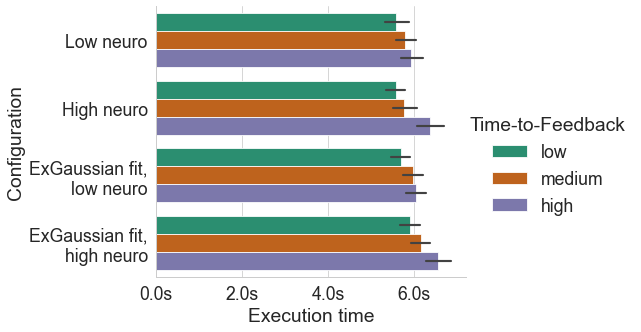
\includegraphics[width=\columnwidth]{figs/new_model/ttf_to_exectime.png}
    \caption{%
        Effects of feeding three different \acp{TTF} (\emph{low}, \SI{0}{\second}, \emph{medium}, \SI{2.5}{\second}, or \emph{high}, \SI{5}{\second}) into the model on the generated execution times.
        Higher \acp{TTF} directly lead to higher execution times.
        Error bars indicate the \SI{95}{\percent} \ac{CI}.
    }\label{fig:ttf_to_exectime}
\end{figure}

\cref{fig:ttf_to_exectime} shows the mean execution time outputted by the model when fed three different levels of \ac{TTF} (\emph{low}, \SI{0}{\second}, \emph{medium}, \SI{2.5}{\second}, or \emph{high}, \SI{5}{\second}).
These results were generated by first warming up the model by feeding it \num{25} \acp{TTF} selected at random from the data before feeding it the desired input \ac{TTF}, and recording the generated execution time.
This procedure is repeated \num{600} times for each configuration and target \ac{TTF}.
The resulting mean execution times match precisely the desired behavior mentioned in \cref{it:ttftoexectime}, with the difference in mean execution times at low versus high \acp{TTF} reaching \SI{14}{\percent} (\textasciitilde\SI{5.6}{\second} to \textasciitilde\SI{6.4}{\second}) in the worst case (high neuroticism configuration).
Additionally, we can observe the effects of neuroticism on generated execution times, as specified in \cref{it:neuro}.
At low neuroticism, the average difference between execution times at low versus high \acp{TTF} was of roughly \SI{6.2}{\percent}, compared to \SI{12.5}{\percent} at high neuroticism.

\begin{figure}
    \centering
    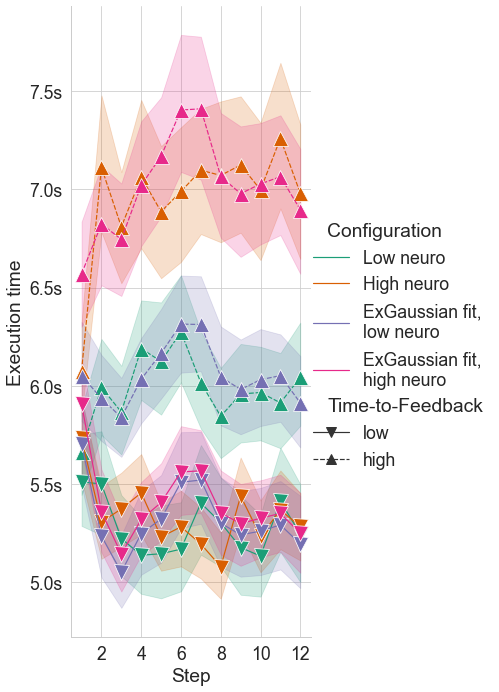
\includegraphics[width=\columnwidth]{figs/new_model/exectime_over_steps.png}
    \caption{%
    Effects of prolonged exposure to constant levels of system impairment on the model.
    At low (\SI{0}{\second}) \ac{TTF}, the models speed-up over time; conversely at high (\SI{5.0}{\second}) \ac{TTF}, the models either present no change or drastically increase their generated execution times, depending on the level of neuroticism.
    Error bars indicate \SI{95}{\percent} \ac{CI}.
    }\label{fig:exectimeduration}
\end{figure}

Next, \cref{fig:exectimeduration} shows the evolution of generated execution times while the model is subject to a fixed \ac{TTF}, either \emph{low} (\SI{0}{\second}) or \emph{high} (\SI{5}{\second}).
These results were generated by first warming up the model with \num{25} random \acp{TTF}, and then recording the generated execution times over a sequence of \num{12} steps at a fixed \ac{TTF}; this procedure is repeated \num{600} times for each configuration and target \ac{TTF}.
Once again, we see here behavior matching what is expected of the model, in particular with respect to \cref{it:duration}.
At low \acp{TTF}, the model is on average, across all configurations, \SI{8.2}{\percent} faster at step \num{12} when compared to step \num{1}.
At high \acp{TTF}, the behavior changes depending on the level of neuroticism of the model.
Low neuroticism models basically do not change their execution times, whereas high neuroticism configurations are on average \SI{10}{\percent} slower after \num{12} steps.
This is once again in line with our previous findings, as we had previously concluded that humans tend to speed up during a task, but that this speed-up is hindered and eventually reversed as system responsiveness decreases, and that the strength of this effect is correlated with neuroticism.

\begin{figure*}
    \centering
    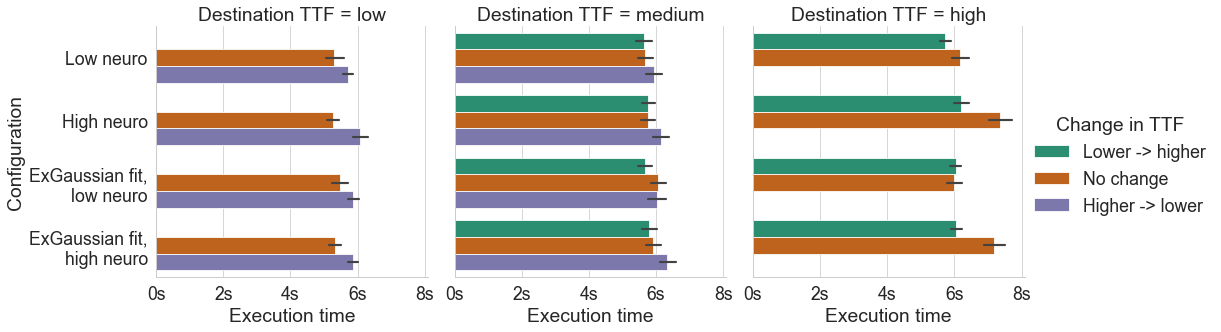
\includegraphics[width=\textwidth]{figs/new_model/transitions.png}
    \caption{%
        Effects of changes in system impairment on subsequently generated execution times.
        These effects linger on after the change, and thus execution times immediately after a transition are either consistently lower or higher than otherwise at the new \ac{TTF}, depending on the old \ac{TTF}.
        Error bars indicate \SI{95}{\percent} \ac{CI}.
    }\label{fig:transitions}
\end{figure*}

Finally, in \cref{fig:transitions} we showcase the behavior of the model when comparing execution times generated immediately after a change in system responsiveness.
We generate these results by first warming up the model by feeding it a fixed \ac{TTF} (which we will refer to as the \emph{origin} \ac{TTF}) \num{25} times.
Next, another \ac{TTF} value (the \emph{destination} \ac{TTF}) is fed to the model, and we record the output execution time.
Each sample is tagged according to the relation between origin and destination \ac{TTF}, either lower to higher, higher to lower, or equal.
As before, we run \num{600} repetitions of this procedure for each combination of model configuration, origin \ac{TTF}, and destination \ac{TTF}.
Execution times generated immediately after a transition from a higher \ac{TTF} into a lower one are consistently higher than execution times generated without a preceding change in \acp{TTF}.
Conversely, execution times are consistently lower than otherwise immediately after a change from a lower \ac{TTF} into a higher one.
These results are once again in line with our findings in~\cite{olguinmunoz:impact2021}, in which we found lingering effects of transitions between levels of system impairment on human execution times.


\subsection{Generating realistic samples}\label{ssec:model:frames}

Apart from the aforementioned timing and performance data, for~\cite{olguinmunoz:impact2021} we also recorded all collected video frame samples together with matching metadata.
For each video frame submitted to the \ac{WCA} during the tasks, we recorded
\begin{enumerate*}[itemjoin={{; }}, itemjoin*={{; and }}]
    \item the raw video frame captured
    \item sample submission timestamp
    \item \ac{WCA} processing completed timestamp
    \item result or acknowledgement returned timestamp
    \item a tag representing the result of the \ac{WCA} processing
\end{enumerate*}.
The tags assigned corresponded to:
\begin{description}[font={\bfseries\ttfamily}, wide]
    \item[SUCCESS:] frames which triggered a transition to a new step (or the correction of a previous mistake) in the logical task model of the \ac{WCA}, and thus cause the generation of feedback to the user.
    \item[REPEAT:] frames which captured the same board state as the previous successful frame, and thus produced no feedback.
    \item[LOW\_CONFIDENCE] frames for which the image recognition algorithm in the \ac{WCA} did not reach the necessary confidence threshold to interpret it as a valid board state.
        These frames also produce no feedback.
    \item[BLANK] frames in which not enough of the board is visible due to noise, movement, occlusion, etc.
        These frames produce no feedback either.
    \item[TASK\_ERROR] frames which contained an incorrect board state and thus triggered a transition to a procedural corrective step and the generation of feedback to the user.
        However, it must be noted that none of the \num{40} participants made any mistakes during the task, and thus no such frames were encountered in the data.
\end{description}

We correlate this frame data with the step timing data described in \cref{ssec:model:exectimes} to match frames with their corresponding step execution times.
We assign to each frame a normalized instant value \( t_\text{norm} \) corresponding to its capture instant \( \tau \) (expressed in seconds since the start of the step) divided by the total execution time \( t_\text{exec} \) of the step:

\begin{align}
    \left( t_\text{norm} = \frac{\tau}{t_\text{exec}} \right) \in [0, 1]\label{eq:tnorm}
\end{align}

% To exemplify, for a step with execution time \( t_\text{exec} = \SI{10}{\second} \), a frame captured at time \( \tau = \SI{3}{\second} \) from the start of the step, will have a normalized instant value \( t_\text{norm} \):
% \begin{align}
%     t_\text{norm} = \frac{\tau}{t_\text{exec}} = \frac{\SI{3}{\second}}{\SI{10}{\second}} = 0.3
% \end{align}

This allows us to analyze the distribution of frame tag probabilities as a step progresses, independently of execution times.
This is illustrated in \cref{fig:frameprobs}.
Intuitively, \texttt{REPEAT} frames dominate the early instants after a step transition, as the user has not had time to start performing the new instruction and thus the \ac{WCA} keeps capturing frames representing the previous state of the board.
As the user starts moving and performing actions, \texttt{BLANK} frames start to dominate, as this activity prevents the \ac{WCA} from capturing ``clean'' frames.
Finally, it must be noted that \texttt{SUCCESS} frames are not included in this probability density plot, as, by definition:
\begin{equation}
    P(\text{\texttt{SUCCESS}} | t_\text{norm}) =
    \left\{ \begin{array}{ll}
        0 & t_\text{norm} < 1.0    \\
        1 & t_\text{norm} \geq 1.0
    \end{array} \right.
\end{equation}

That is, any frame captured immediately at or after the execution time has been reached will contain the finished board state and thus correspond to a \texttt{SUCCESS} frame.

\begin{figure}
    \centering
    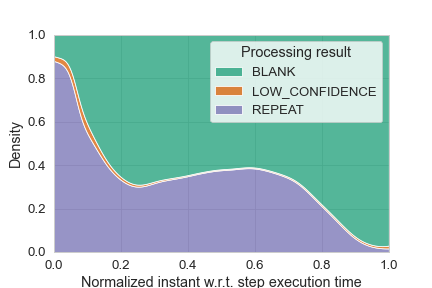
\includegraphics[width=\columnwidth]{model_data/frame_probabilities.png}
    \caption{%
        Probability density of frame result tags as a step progresses.
        Note that \texttt{SUCCESS} frames are not included as --- by definition --- the probability for success frames is \num{1} for all normalized instant values greater than or equal to \num{1.0}.
    }\label{fig:frameprobs}
\end{figure}

Using the above insights, together with the corresponding recorded video frames, we devise a scheme for the procedural generation of a synthetic trace for any step in \ac{WCA} task in the same category as those used in~\cite{olguinmunoz:impact2021}.
We first prepare a discretized representation of the probability density map in \cref{fig:frameprobs}.
We segment the normalized instant value into a number of discrete bins (\num{25} in this work), and calculate the relative fraction of frames for each category in each bin.
For each step, given
\begin{enumerate*}[itemjoin={{; }}, itemjoin*={{; and }}]
    \item a collection of random non-\texttt{SUCCESS}, non-\texttt{REPEAT} frames (at least one frame for each of the \texttt{BLANK} and \texttt{LOW\_CONFIDENCE} categories)
    \item an appropriate \texttt{SUCCESS} video frame containing the correct state for the step
    \item an appropriate \texttt{REPEAT} video frame containing the correct state for the \emph{previous} step
\end{enumerate*},
we can then procedurally generate a trace by randomly selecting appropriate frames according to the distributions presented in \cref{fig:frameprobs}.
In other words, for each sampling instant in a step with a given execution time \( t_\text{exec} \):
\begin{enumerate}
    \item We calculate \( t_\text{norm} \) according to \cref{eq:tnorm}.
    \item If \( t_\text{norm} \ge 1.0 \), we select the \texttt{SUCCESS} frame and stop sampling.
    \item If instead \( t_\text{norm} < 1.0 \), we find the appropriate bin for \( t_\text{norm} \) and then select a frame by performing a weighted random sampling of the frame categories in the normalized instant bin.
\end{enumerate}

\subsection{Obtaining the model}\label{ssec:model:obtaining}

We provide the model implementations in Python~\num{3.10} as well as the base data to the community as \ac{FOSS}.
All of these are published on the \href{https://github.com/KTH-EXPECA/EdgeDroid2}{\texttt{KTH-EXPECA/EdgeDroid2}} repository on GitHub under a permissive Apache version 2 license.